\section{Phoenix}
\label{sec:previous_work}
\textsc{Phoenix} is divided into three main modules:
\begin{description}
  \item[\textbf{DGA Discovery Module}] \hfill \\ is responsible of separating AGDs from HGDs;
  \item[\textbf{DGA Detection Module}] \hfill \\ is responsible of labeling the AGDs, matching them
    to a specific DGA;
  \item[\textbf{Intelligence and Insights Module}] \hfill \\ aggregates, correlates and monitors the
    results of the other modules to extract meaningful insights~\cite{Lorenzo2013}.
\end{description}

In the next sections we shall briefly describe the DGA Discovery and the DGA Detection module.

\subsection{DGA Discovery Module} % (fold)
\label{ssub:dga_discovery_module}
This module is further divided into three steps.
\begin{description}[\leftmargin 0.5\parindent]
  \item[\textbf{AGD Filtering}] \hfill \\
    During this phase \textsc{Phoenix}, provided with a set of malicious domains,
    computes a four elements feature vector which exploits four linguistic characteristics
    to separate AGDs from HGDs;
  \item[\textbf{AGD Clustering}] \hfill \\
    It receives a set of possible AGDs from the previous step. Then, it tries to
    produce clusters based on the IPs the domains resolve to.
  \item[\textbf{DGA Fingerprinting}] \hfill \\
    It extracts from each previously discovered cluster five cluster features, in order
    to fingerprint the DGA, as to be able successively label unseen domains.
\end{description}
% subsubsection dga_discovery_module (end)

\begin{figure*}[h!tp]
  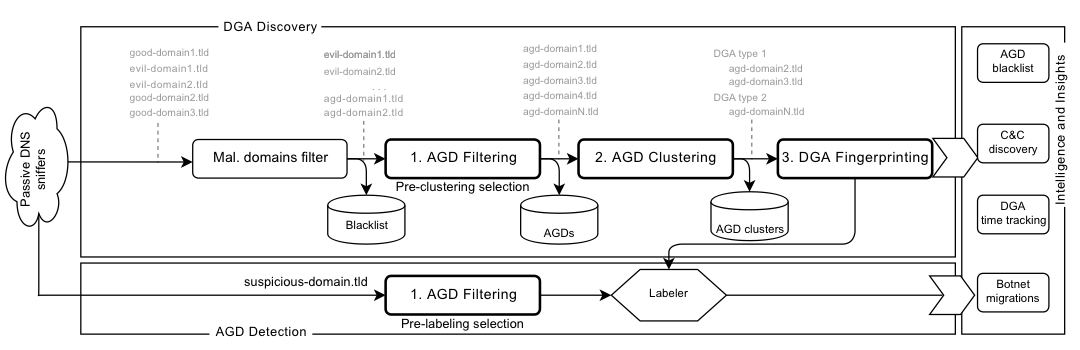
\includegraphics[width=\textwidth]{phoenix.png}
  \caption{The \textsc{Phoenix} modules.}
  \label{fig:phoenix}
\end{figure*}

\subsection{DGA Detection Module} % (fold)
\label{ssub:dga_detection_module}
The DGA Detection Module receives a previously unseen domain name. It determines
whether it is automatically or human generated, by running the filtering step of the
DGA Discovery Module. If this is the case, its features are computed and matched
against the fingerprints obtained before.
% subsubsection dga_detection_module (end)
% section previous_work (end)
